\documentclass{article}
\usepackage{a4wide}
\usepackage[dvipsnames,svgnames]{xcolor}
\usepackage[pdftex]{graphicx}
\usepackage{enumitem}
\usepackage{lscape}
\usepackage[a4paper]{geometry}
\usepackage{pdfpages}

\begin{document}

\title{Group project in TDT4215\\
Web-intelligence}

\date{April 20, 2013}

\author{
  Alessio DE ANGELIS\and 
  Martin HENGSTBERGER\and
  Simon STASTNY}

\maketitle

\tableofcontents
\newpage


\section{Introduction}

This report was created during the Web- Intelligence (TDT4215) course in the spring semester of 2013. It contains information about the mandatory group project. The task was to, automatically suggest relevant treatments and drugs by using doctor's patient notes and an electronic handbook for pharmaceutical interventions. A java application was created using several tools as well as a lot of creativity. You can find a description of the application's architecture, the processing, the limits and the results of the Project. Finally we analyze the results and collect some ideas how to improve the application.

\section{System architecture}

Since the nature of most of the tasks in this software system is highly time consuming, we decided to take advantage of provided multithreading facilities that Java offers and we implemented the software using Java Executor Framework. This choice made the code a bit more complicated than a code of regular single-threaded application, but we managed to reduce the execution time significantly on multi-processor machine.\footnote{Execution time on a machine with Intel Core i3 (M350 2.27GHz) was reduced by a factor of cca 3.}

Given the fact that our main architectural drivers were short time to market and developer inexperience, we decided to use just basic facilities of chosen frameworks and tools. Spending too much time learning details of tools such as \emph{Jena} and \emph{Lucene} would leave with a little time to make the actual implementation.

As stated above, we are using some tools such as \emph{Jena} and \emph{Lucene}. Their particular use in the application is described below in corresponding chapters. Apart from those tools, we are for example using SAX and Apache Tika for parsing tasks.

\section{Components function and role}
Many tasks occuring in the application share some similarities in behaviour and structure and thus we made the system very modular and easily modifiable. The sequence diagram shown in \ref{fig:seq} displays a naive view over the system. Please note, that \texttt{Indexer}, \texttt{Parser} and \texttt{QueryEngine} are general names for different implementations (ATC files are parsed and indexed differently than ICD files, however the structure of the software component is similar).

\begin{figure}[h!]
    \label{fig:seq}
    \centering
    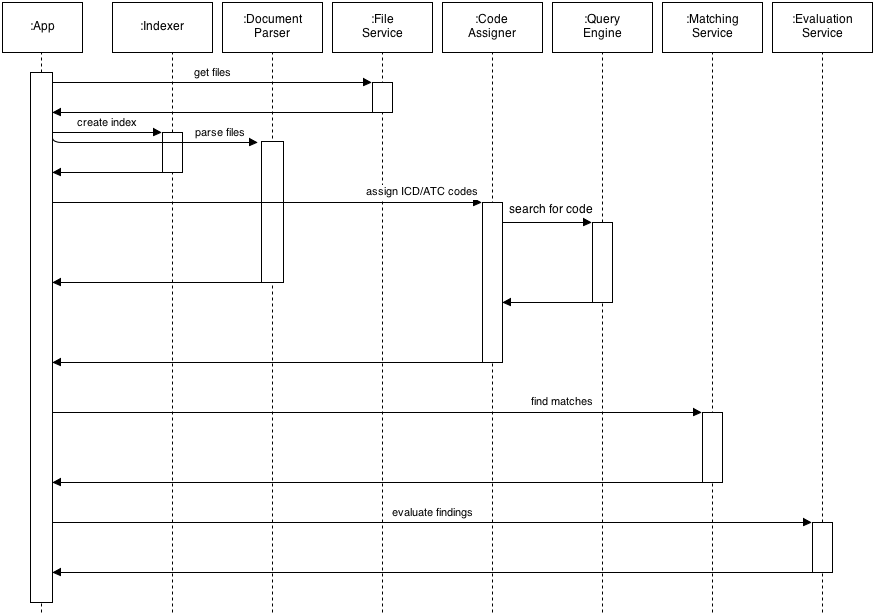
\includegraphics[width=1.0\textwidth]{seq}
    \caption{Sequence diagram}
\end{figure}

\begin{figure}[h!]
  \centering
    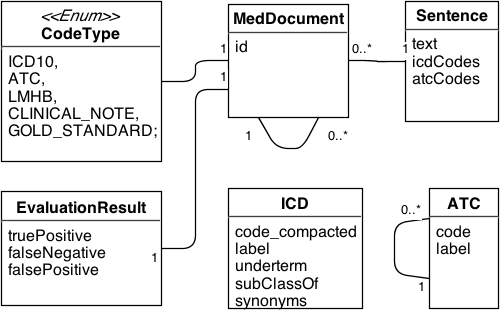
\includegraphics[width=1.0\textwidth]{class}
    \caption{Class diagram}
\end{figure}

\subsection{Parsing ICD and ATC files}

There are several ways to parse ICD and ATC files to extract information from them: you can consider those as normal XML files, use regular expressions and so on.

We have chosen a semantic web tool, \emph{Jena}.\footnote{http://jena.apache.org/} As we can read from the website: \emph{Jena is an API for reading, processing and writing RDF data in XML, N-triples and Turtle formats; an ontology API for handling OWL and RDFS ontologies; a rule-based inference engine for reasoning with RDF and OWL data sources; stores to allow large numbers of RDF triples to be efficiently stored on disk}. 

This tool may seems to be a little bit verbose to use, but it lets us handle in a very efficient way both the ontologies, the ICD that is an OWL format and the ATC that is a turtle, without the risk of losing information from them. Moreover, we can have easily access the information about all the rdf graphs: we can keep track for example of the hierarchies, the subclasses, the synonyms and so on. All this extra information may be used to improve our query engine, doing some refinements when the pure textual search is not accurate enough.

When we parse ICDs we store them in java beans the values of the following properties \texttt{code\_compacted} (the code of the disease), \texttt{label} (description of the disease), \texttt{underterm} (extra information about the disease, not every instance has it), \texttt{synonyms} and \texttt{subClassOf}.
When we parse ATCs we store them in java beans the values of the code, the \texttt{label} and \texttt{subClassOf}.

\subsection{Tools for indexing and querying}
For indexing and querying we are using an information retrieval approach, through a bag of words model. We are using \emph{Lucene} \footnote{http://lucene.apache.org/core}. We read from the Website:\emph{Apache Lucene\TM is a high-performance, full-featured text search engine library written entirely in Java. It is a technology suitable for nearly any application that requires full-text search, especially cross-platform.} Lucene is scaleable, powerful and accurate for using efficient search algorithims.
At the beginning we were trying to create our own information retrieval engine, but we came across several problems. First of all how to deal with Norwegian language, our background is very poor since we are all international students in the group, how to stem correctly words or divide properly the \emph{aggregates} (four, five words merged all together in one). \emph{Lucene} is a library made by experts and their implementation of the \texttt{NorwegianAnalyzer} (with the Porter stemming algorithm), even if maybe not as accurate as the English one, has been revealed very useful for our purposes. Moreover it natively supports the vector space model for a more accurate retrieval than boolean.

We keep two different indexes, one for the ATC documents and the second for the ICD documents. Since the indexing is very fast, we keep both the indexes in ram, for performance reasons during the queries (you don't need to access the disk that is usually time consuming). The ATC documents are composed by two fields: one for the atc\_code, that just indexed without any further string processing; the second field, \texttt{label}, contains the description of the code and is the one used for extracting the documents. This field is indexed, stored, tokenized and calculates the term vector matrix.

The ICD documents are indexed according to three fields. The first one is for the property \texttt{icd:code\_compacted}, to identify uniquely the codes. The second one is for the \texttt{label:} the field has the same properties as the ATC label. The third field contains all the terms of the label plus the other information for doing query expansion, such as the synonyms and the property \texttt{icd:underterm}. Adding those extra words let have a more accurate result when we submit the query to our engine. In fact at the moment we query the ICD index looking into the terms contained in the extra field.

\subsection{Parsing patient cases}

Since the assignment description states that preprocessing of patient case input file is legal, we took the chance and manually made an XML file representing the data contained in the \texttt{.doc} file provided. Parsing a \texttt{.doc} file would be a waste of time with no learning outcome. This as well gave us the opportunity to decide how the text is divided into sentences manually.

To parse this created XML document, we were using SAX parser with our own implementation of the \texttt{DefaultHandler} to produce \texttt{MedDocument} instances from the files read. This part of the work gets done in \texttt{PatientCaseParser}.

\subsection{Parsing the gold standard file}

To perform the evaluation easily, we decided to make an XML file for the gold standard file\footnote{/data/goldStandard.xml} and let the application read and compare it the two result sets (the produced one and the one from gold standard) automatically. This file gets read by \texttt{GoldStandardParser} and data are held as instances of \texttt{MedDocument}.

After the patient case files are read, assigned codes and found their relevant matches from the book, we compare the relevant matches with those from the gold standard. This gets done \texttt{EvaluationService} in the very end of the program run. Evaluation results are then stored in an XML file.\footnote{\texttt{/data/output/evaluation.xml}}

\subsection{Parsing the book}

The headlines in the handbook identify the therapies and drug descriptions. Those are parsed into instances of \texttt{MedDocument} as well as the corresponding text body. The text is spitted into sentences for later processing. Headlines that do not start with a legal (i.e. \textit{T3.1.1} or \textit{L2}) therapy or drug identifier are skipped. The following text is skipped too, until a legal heading is found.
There were challenges with invalid\footnote{http://validator.w3.org/\#validate\_by\_upload} HTM files. Furthermore different ways of encoding special characters were used. I.e. both \textit{"\&aring;"} (HTML entity) and \textit{"\&#x00E5;"} (Unicode) appear.

\section{Limitations given in the assignment. Present theories used. Are any theories outside of the curriculum been used? Explain the reason for the selection}
\section{How have the theories been adapted to the assignment?}
\section{Summary of the results.}
\section{Evaluation and discussion of the results. Limitations of your evaluation results.}
\section{Thoughts of potential improvements.}
\section{Conclusions.}

\section{Future work}
Our system is accurate but in the future some refinements could be done to improve our query engine that we didn't manage to implement due to time constraints. For example an evaluation function that gives more  importance to the hierarchy of the classes, for example if a code is subClassOf another code (E10, subclass and E10-14, the superclass in ICD for example). Since we use \emph{Jena} to read the OWL ontologies, could be done through a simple graph traversal using suitable methods offered by the APIs, or using ad hoc SPARQL queries.

We could even taken better into account the synonyms: if two codes have the same synonyms, the may refer to the same disease.

\end{document}